\documentclass[border=10pt,12pt]{standalone} 
\usepackage{graphicx}
\usepackage{tikz}
\usepackage{xcolor}
\usetikzlibrary{arrows,automata,decorations,chains,fit,quotes,shapes,positioning,calc}


\begin{document}

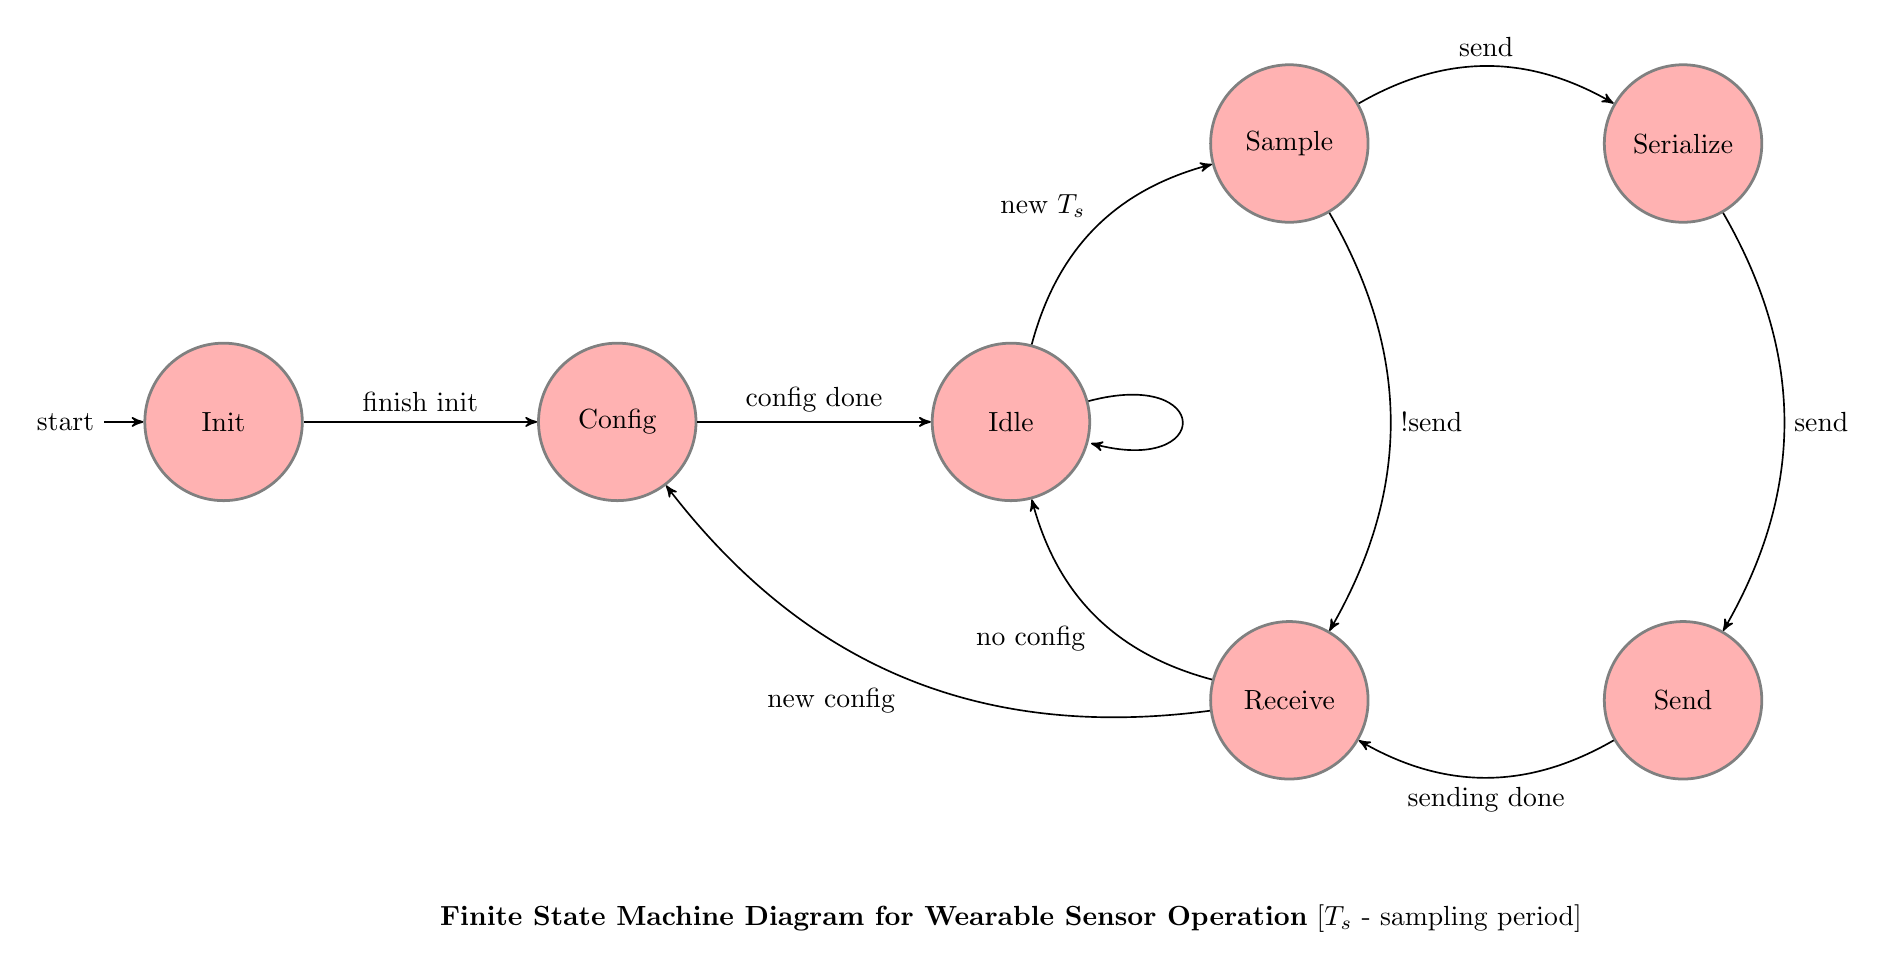
\begin{tikzpicture}[->,>=stealth',auto,node distance=5cm, semithick, transform shape, align=center,on grid,auto]

    \tikzstyle{every state}=[draw=gray,line width=1pt,circle,fill=red!30,text=black,minimum size=2cm]
    
    \node[initial, state, initial distance=.5cm] (A)    {Init};
    \node[state] (B) [right of = A]                     {Config};
    \node[state] (C) [right of = B]                     {Idle};
    \node[state] (D) [above right of = C]               {Sample};
    \node[state] (E) [right of = D]                     {Serialize};
    \node[state] (G) [below right of = C]               {Receive};
    \node[state] (F) [right of = G]                     {Send};

    \path (A) edge              node                        {finish init}   (B)
          (B) edge              node                        {config done}   (C)
          (C) edge [bend left]  node                        {new $T_s$}     (D)
              edge [loop right] node                        {}              (C)    
          (D) edge [bend left]  node                        {send}          (E)
              edge [bend left]  node                        {!send}         (G)
          (E) edge [bend left]  node                        {send}          (F)
          (F) edge [bend left]  node                        {sending done}  (G)
          (G) edge [bend left]  node                        {no config}     (C)
              edge [bend left]  node                        {new config}    (B);
    
    \node [below=6cm, align=flush center,text width=20cm] at (C) {\textbf{Finite State Machine Diagram for Wearable Sensor Operation} [$T_s$ - sampling period]};
\end{tikzpicture}
\end{document}